\chapter{Implementation}\label{Ch:Implementation}
\section{General}
The autonomous landing system for stationary net landing consist mainly of three modules, which is the Navigation, LandingPlan, and Path Controller tasks. A simplified figure of the system flow in the autonomous landing system in \gls{dune} is showed in figure \ref{fig:DuneSystem}. The implementation and system description of the path controllers used in the autonomous landing system is not a focus area in this thesis, however a short description is given in appendix \ref{AP:ControlGuidanceSystem} and a closer analyse of the path control system can be found in the master thesis \citep{Sigurd}. The \gls{dune} task Ardupilot is used as interface towards the Ardupilot software which either runs as in a simulation mode or on a Pixhawk. The gls{dune} system is command  and controlled with Neptus, which has been modified to suit the needs of the autonomous landing system.
\begin{figure}[H]
	\centering
		\includegraphics[scale=0.8]{figs/DUNESystem.png}
		\caption{A simplified depiction of the interaction between the major components in the autonomous landing system during stationary net landing}
		\label{fig:DuneSystem}
\end{figure}
\section{Navigation system}\label{IMP:NavSys}
The navigation state control system described in section \ref{S:NavState} is implemented in the \gls{dune} task Navigation. This \gls{dune} task is used to control the position and velocity information source of the navigation state \gls{imc} message EstimatedState. Depending on the current state of the navigation system the \gls{imc} EstimatedState message will either have position solution form the \gls{rtk-gnss} system or the external navigation system. During a short loss of the \gls{rtk-gnss} the external navigation position is compensated with the average difference between the \gls{rtk-gnss} solution and the external navigation solution. The state of the navigation system is monitored through the \gls{imc} message NavSources, which contain the information about the source of the state information, including which alternative navigation system is available for the \gls{uav} navigation system.
\subsection{RTK-GPS system}\label{ss:RTK-GPS system}
The \gls{rtk-gnss} solution is made available to the DUNE system through the \gls{dune} task RTKGPS, which is an modified version of the same \gls{dune} task developed in the master thesis \citep{Spockeli}. The \gls{rtk-gnss} solution is included in the \gls{imc} GpsFixRtk message, however in order for the message to be valid the following flags must be set true:
\begin{table}[H]
\begin{itemize}[noitemsep]
\item Valid velocity
\item Valid position
\item Valid time
\item Valid base
\end{itemize}
\end{table}
The three first flags are set automatically when receiving a output solution from RTKLib, however since the base station position is not included in the RTKLib output the valid base flag will not be set automatically. In order for the GpsFixRtk message in the \gls{uav} to get a valid base station position, the base station must calculate it's own position and send it to the \gls{uav}. Figure \ref{Fig:ValidationGpsFixRtk} shows the message flow which is needed in order for the GpsFixRtk message in the \gls{uav} to be considered valid by the \gls{uav} navigation system. The \gls{dune} task basestationFix must be reconfigured that the base station position is fixed from Neptus in order for the base station to start transimiiting its own position to the \gls{uav}. The advantage with a fixed base station position in the \gls{dune} system is that all vehicle that uses \gls{rtk-gnss} will be in the same reference frame, which enable high accurate vehicle coordination.
\begin{figure}[H]
\centering
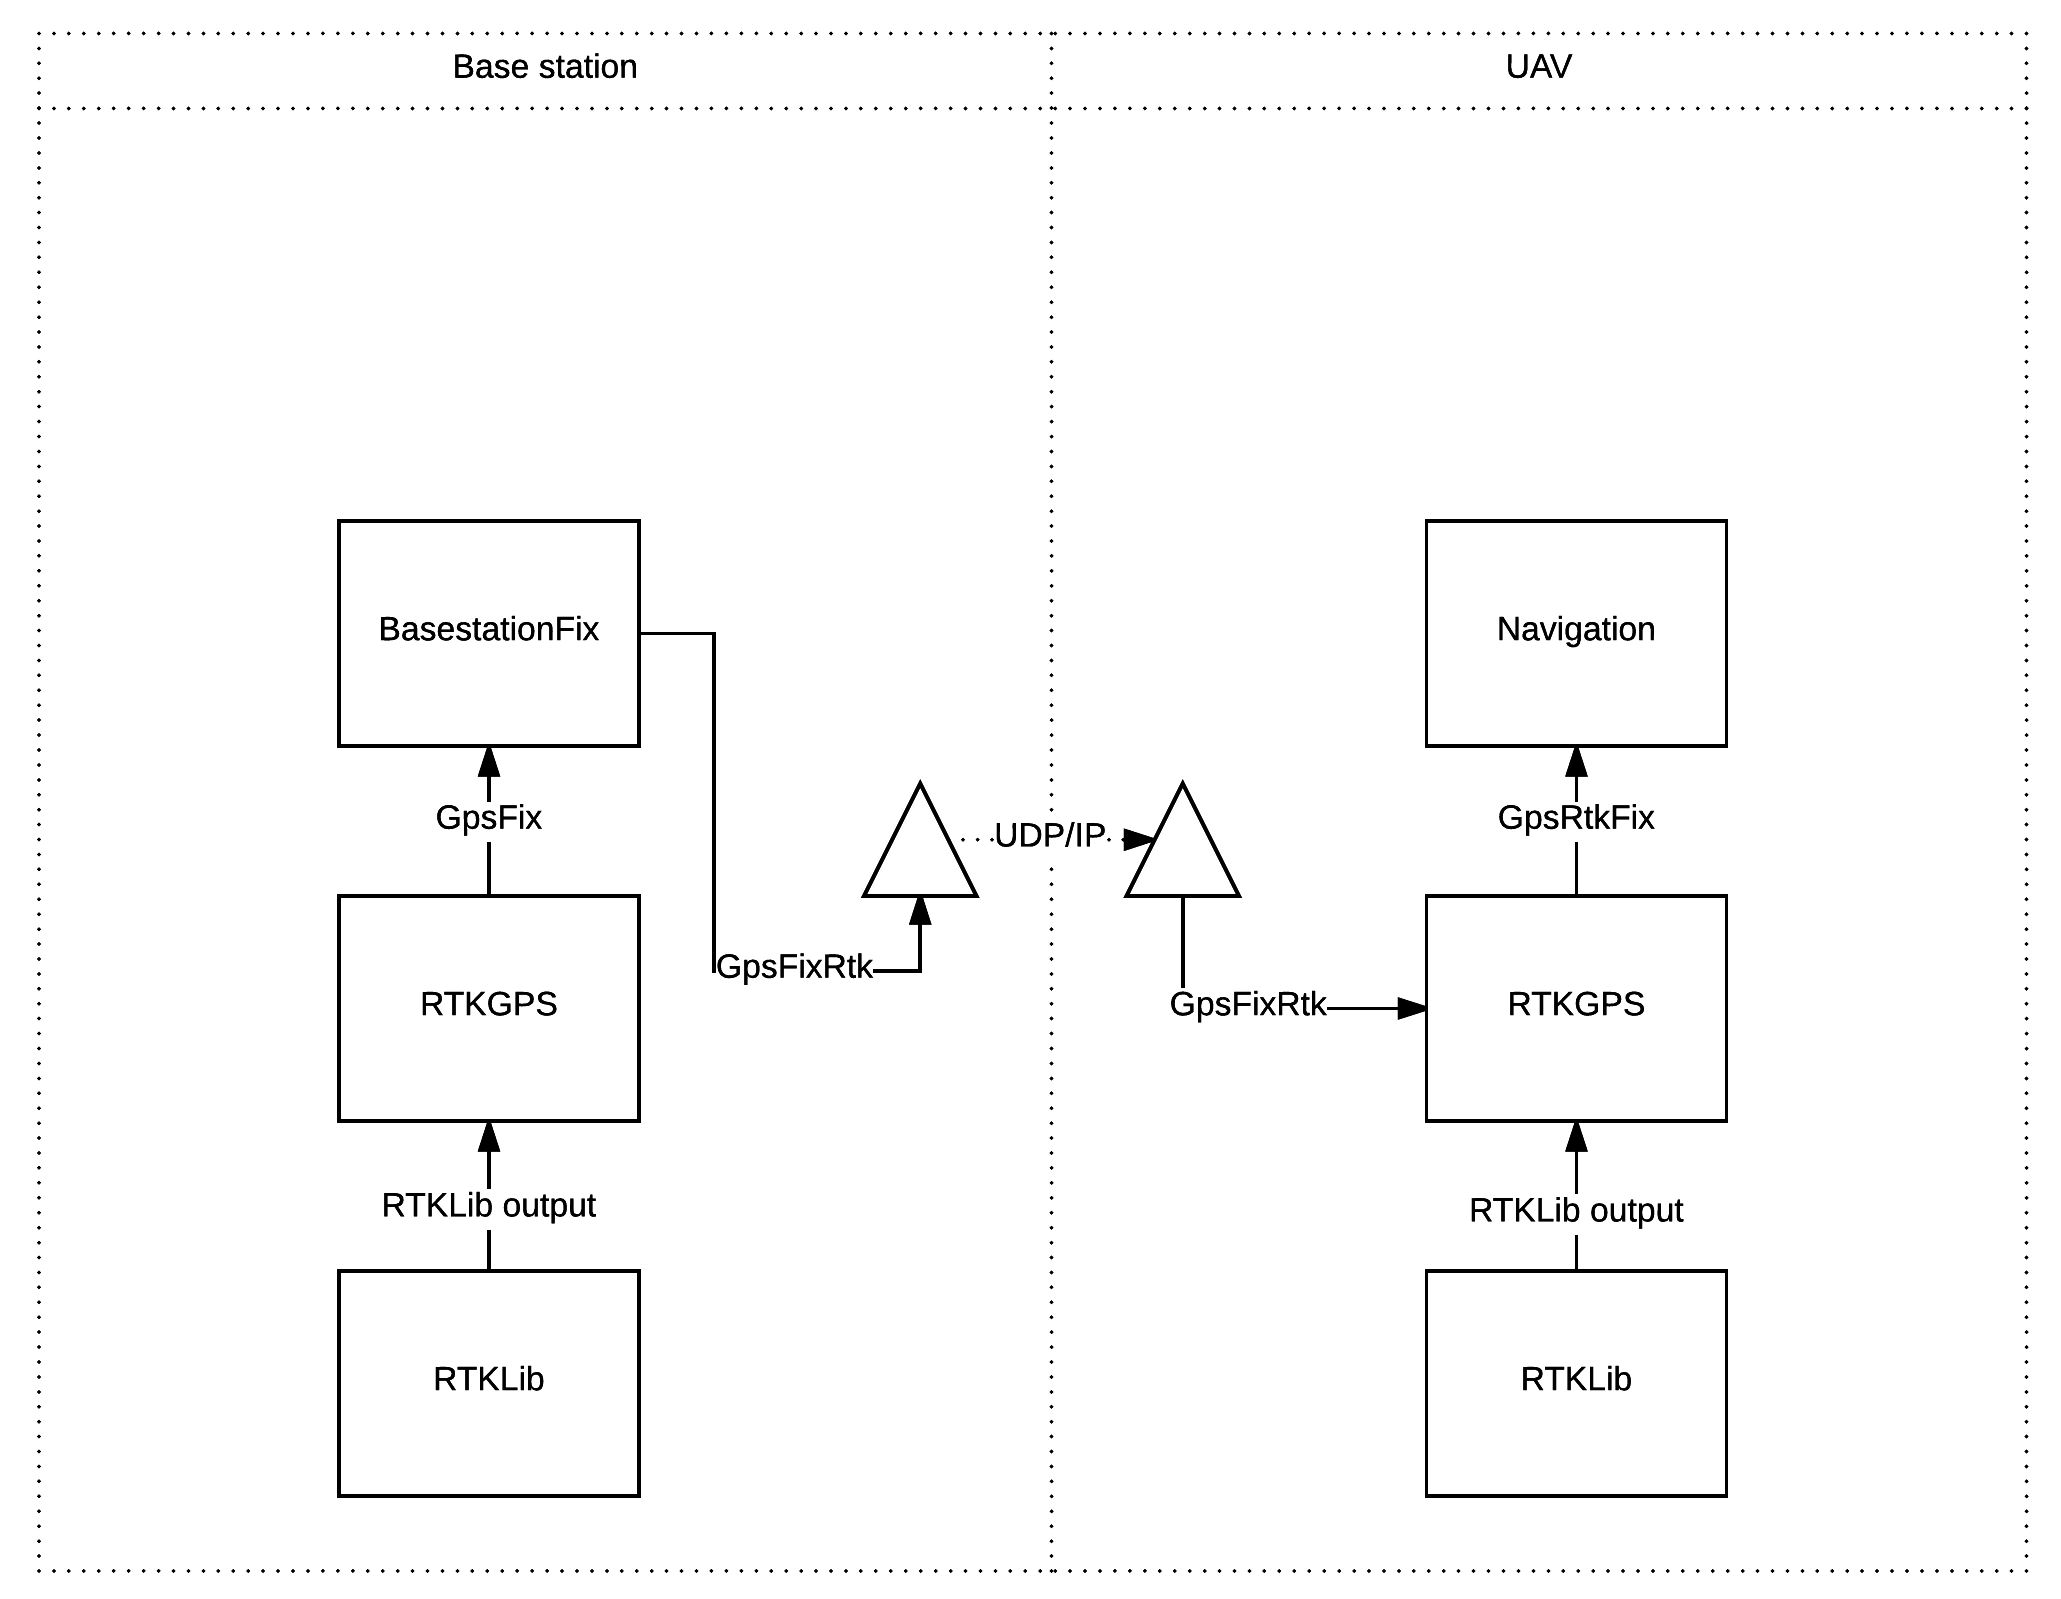
\includegraphics[scale=0.7]{figs/ValidationGpsFixRtk.png}
\caption{Message flow for validation of GpsFixRtk}
\label{Fig:ValidationGpsFixRtk}
\end{figure}
\subsection{Navigation state control system}
The navigation state control system described in section \ref{S:NavState} is implemented in the \gls{dune} task Navigation. Figure \ref{Fig:NavStateControlFlow} shows the system flow in the navigation state control system, which is trigger by either receiving a ExternalNavData or GpsFixRtk \gls{imc} message. Both types of messages is stored internally in the DUNE task, however the GpsFixRtk is used to trigger update of the short rtk loss compensator. The state machine performs its state transition action while entering the new state. The state change will then trigger an alteration in the content of the EstimatedState \gls{imc} message whether the position and velocity information should be from \gls{rtk-gnss} or from the external navigation system.

In the case where \gls{rtk-gnss} is lost the short \gls{rtk-gnss} loss compensator described in section \ref{ss:ShortLoss} is implemented in the Navigation task. The compensator is used to prolong the availability of the \gls{rtk-gnss}, however if the Navigation task does not receive a valid GpsFixRtk before the deactivation timer triggers the resulting action from the navigation state control system would be to set the \gls{rtk-gnss} system as unavailable.
\begin{figure}[H]
\centering
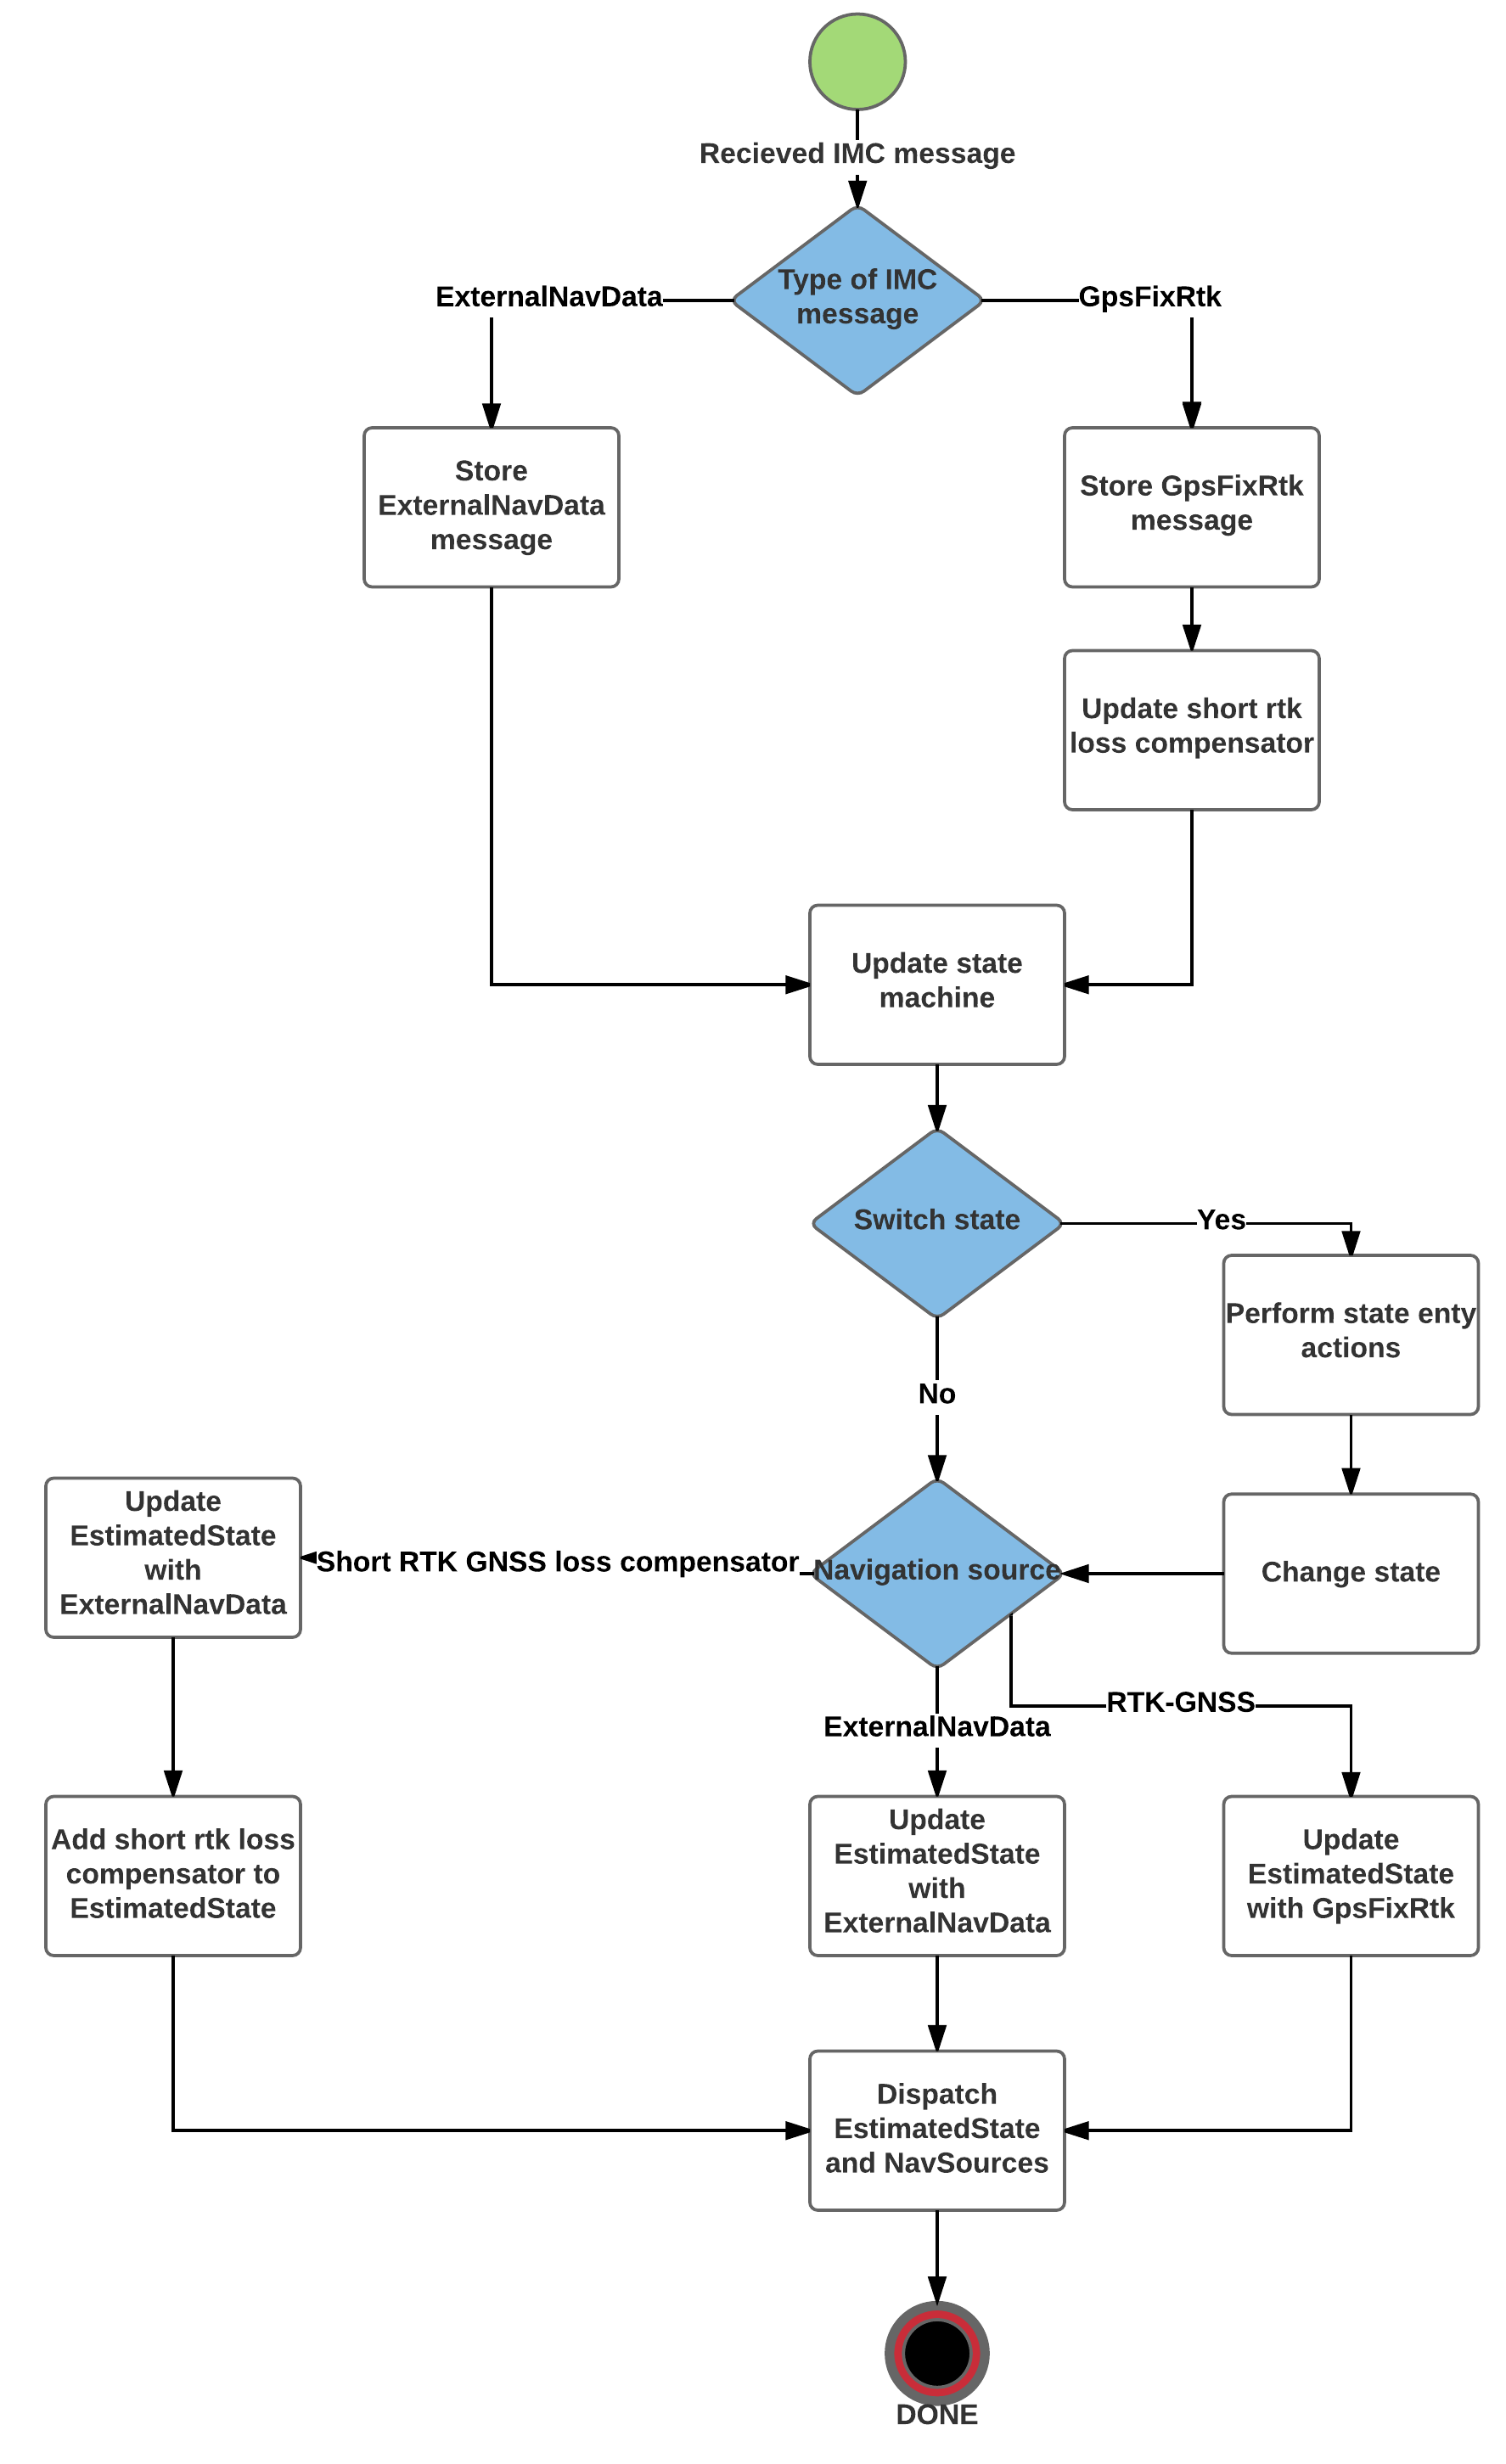
\includegraphics[scale=0.17]{figs/NavStateControl.png}
\caption{Flow chart of the navigation state control system}
\label{Fig:NavStateControlFlow}
\end{figure}
\subsection{Mobile sensor unit}\label{ss:MobileSensor}
The mobile sensor unit is a box that can moved around and act as a reference position for other vehicles in the \gls{dune} systems, e.g. net placement for the autonomous landing system. The mobile sensor unit apply \gls{rtk-gnss} in the same manor as a \gls{uav}, however the mobile sensor unit does not include a external navigation system. Thus a simplified version of the Navigation task has been created for the mobile sensor unit, which is the \gls{dune} task RtkNavigation. The \gls{dune} task RtkNavigation handle the GpsRtkFix message similar to the Navigation task, however due to not having a external navigation system only the GpsFixRtk position solution is used in the EstimatedState message. Figure \ref{Fig:MobileSensor} shows a picture of the mobile sensor unit.
\begin{figure}[H]
\centering
\includegraphics[scale=0.2]{figs/DSC00173.JPG}
\caption{The mobile sensor unit}
\label{Fig:MobileSensor}
\end{figure}
\subsection{Navigation source monitor}
The navigation source monitor is a plug-in in Neptus used to monitor which navigation source a vehicle is using. The monitor consume the NavSources \gls{imc} message, which contain the navigation sources that are currently in use and which are available. The monitor apply a color code to indicate which source is currently in use, in addition to all sensor system that are available. A figure of the navigation source monitor is seen in figure \ref{Fig:NavsourceInterface}, with the color code description given in table \ref{Tb:Color Code}.
\begin{table}[H]
\begin{center}
    \begin{tabular}{ | l | l |}
    \hline
    \textbf{Color} & \textbf{Description} \\ \hline
    White & Not available \\ \hline
    Yellow & Available, but not in use \\ \hline
    Green & Available, and in use \\ \hline
    \end{tabular}
\end{center}
\caption{Net approach parameters }
\label{Tb:Color Code}
\end{table}
\begin{figure}[H]
\centering
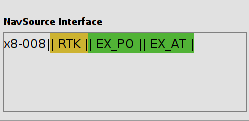
\includegraphics[scale=0.6]{figs/NavSourceInterface.png}
\caption{Navigation source interface}
\label{Fig:NavsourceInterface}
\end{figure}
\section{Landing plan generator}
The \gls{dune} task LandingPlan is the implementation of the landing plan generation system described in section \ref{Ch:LandingPlan}. The \gls{dune} task receive its plan parameter through a \acrfull{api}, which is a \gls{imc} message called LandingPlanGeneration. The task is triggered by the event a LandingPlanGeneration message is consumed, which results in the generation of the approach and landing path. Together the paths form the landing plan. The \gls{api} can be accessed from Neptus through the plug-in LandMayLayer, enabling a graphical interface to be used for net placement.
\subsection{Landing plan generation API}
The landing plan generation \acrfull{api} is a \gls{imc} message used to structure the input parameter used to create the landing plan. With the \gls{api} the desired path parameter can be set, in addition to behaviour setting used to create a specific landing plan. The \gls{api} can be used to set the rotation direction of the start and finish turning circle, by setting the "Automatic" flag to false. In addition a loiter manoeuvre can be added to the landing path, which act as a waiting manoeuvre. The behaviour settings in the \gls{api} are listed in table \ref{Tb:DubinConfig}, with the entire \gls{api} listed in appendix \ref{AP:APIIMC}.
\newpage
\begin{table}[H]
\centering
\begin{tabular}{| p{2.7cm} | p{6cm} |}
\hline
\textbf{Parameter name} 							& \textbf{Description} \\ \hline
 Automatic (boolean)								& If true a standard path where the shortest Dubins path is chosen as the approach path. Otherwise a user specific path is chosen \\ \hline
Start circle turning counter clockwise (boolean)	& If true the start turning circle is created with a turning direction which is counter clockwise. Otherwise clockwise. Require Automatic==false \\ \hline
Finish circle turning counter clockwise (boolean)	& If true the finish turning circle is created with a turning direction which is counter clockwise. Otherwise clockwise. Require Automatic==false \\ \hline
Wait at loiter (boolean)							& If true a unlimited loiter is included into the landing plan. \\ \hline

\end{tabular}
\caption{Landing plan behaviour setting in Landing plan generation \gls{api}}
\label{Tb:DubinConfig}
\end{table}
\subsubsection{Neptus API graphical interface}
In Neptus the plug-in LandmapLayer, which is an altered version of the Neptus plug-in developed in the master thesis \citep{Froelich}, is used to configure the landing plan generation \gls{api}. The alteration in the plug-in includes new parameters, the inclusion of the \gls{imc} message LandingPlanGeneration and the ability to manually write the global position coordinates of the net. The \gls{api} graphical interface which is used in Neptus is shown in figure \ref{Fig:LandMapLayer}. The LandmapLayer plug-in works by first placing the net in Neptus, continued by setting the desired parameters of the landing plan in the graphical interface.
\newpage
\begin{figure}[H]
\centering
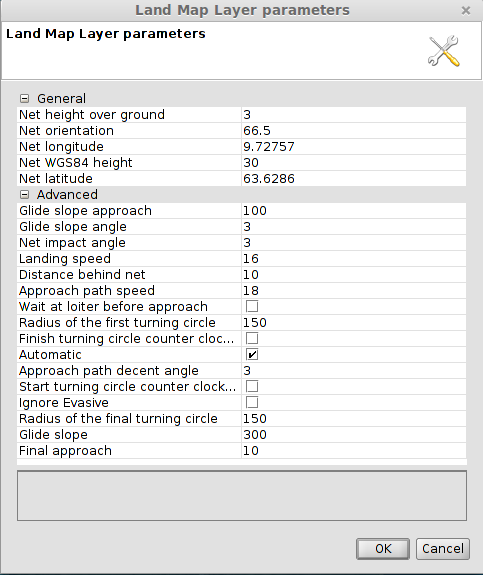
\includegraphics[scale=0.6]{figs/LandMapLayer.png}
\caption{Graphical interface for the landing plan  generator \gls{api} in Neptus}
\label{Fig:LandMapLayer}
\end{figure}
\subsection{Approach path}
The approach path described in section \ref{SS:LandingApproach} is implemented in the \gls{dune} task LandingPlan, where the start position of the approach path is the initial position of the fixed wing \gls{uav} at the time the LandingPlanGeneration message is sent. The final position of the approach path is the first $\textbf{WP}$ in the landing path. Figure \ref{Fig:FlowChartApproach} shows the structure of the creation of the approach path in the landing plan. The creation is trigger by the consumption of a LandingPlanGeneration message, which is extracted in order gain access to the landing plan parameters. 

The creation of the approach path is designed to enable the user to specify the rotation direction of the start and finish turning circles. This design choice was made such that the user has a guaranty of the turning direction in both circles, which is not given when calculating the shortest Dubins path. Thus the two mode have different guaranties, such that the landing plan generator becomes more flexible. 

\begin{figure}[H]
\centering
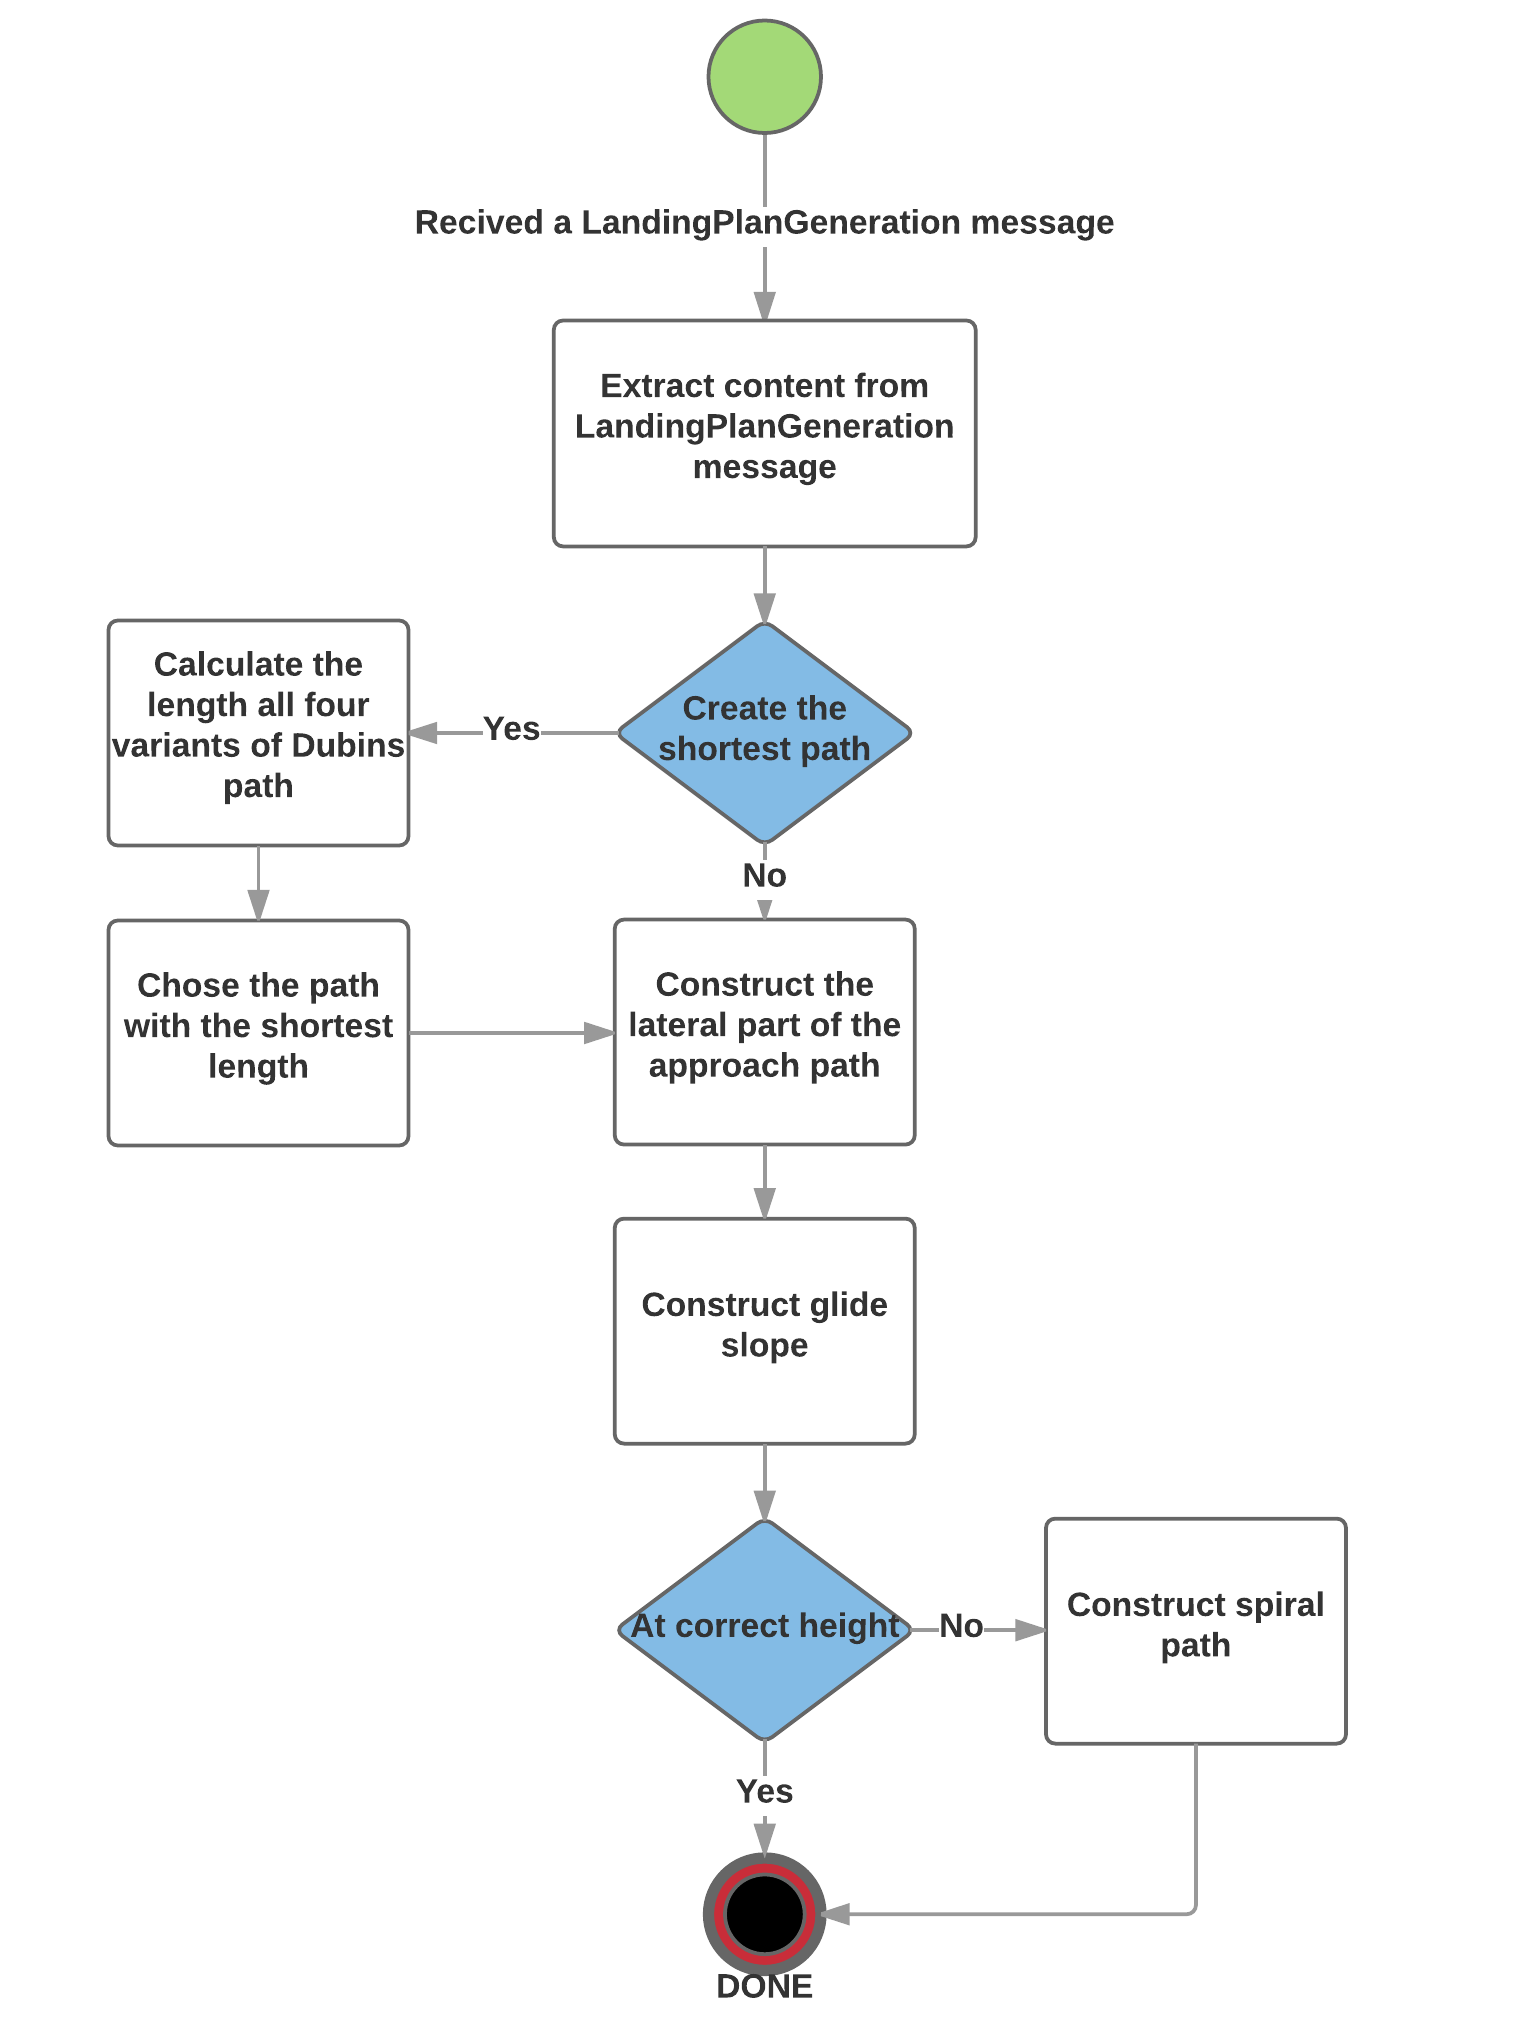
\includegraphics[scale=0.8]{figs/ApproachPath.png}
\caption{Flow chart of approach path creation}
\label{Fig:FlowChartApproach}
\end{figure}
The approach path is created as a FollowPath manoeuvre, which is a manoeuvre where each point in the manoeuvre is defined relative to a fixed reference position. This manoeuvre is suited for more complex manoeuvres, which is the reason it's used in the approach path. The task configuration parameter "Distance Between Arc Segments" is used to specify the distance between each point in both the turning circles, thus given the total number of segments in the circles. The parameter can be used to increase the performance of the lateral control system, by continues switching point to create a smoother circle. The default value of the configuration parameters "Distance between Arc Segments" is given in table \ref{Tb:LandingPlanParameter}.
\begin{table}
\centering
\begin{tabular}{| p{5cm} | p{1cm} | p{5cm} |}
\hline
\textbf{Configuration parameter name}	& \textbf{Default value}	& \textbf{Description} \\ \hline
Distance Between Arc Segment			& $ 25 m$					& Distance between each arc segments in the turning circles \\ \hline
\end{tabular}
\caption{Configuration parameter for the landing plan}
\label{Tb:LandingPlanParameter}
\end{table}
\subsection{Landing path}
The landing path described in section \ref{SS:netApproach} is implemented in the \gls{dune} task LandingPlan, where the path is created relative to the position and heading of the net retrieved from the LandingPlanGeneration message. Figure \ref{Fig:FlowChartLanding} shows the system flow for the creation of the landing path. The creation is trigger when the approach path has successfully been created. A option for the landing path is that it includes a loiter manoeuvre at the beginning, which is defined as a circular manoeuvre around a fixed position with a constant radius. The loiter manoeuvre increase the flexibility of the autonomous landing system, by introducing a manoeuvre in which the \gls{uav} can wait for the landing zone to be prepared. In the case of a dynamic net landing the loiter manoeuvre can be used as a waiting manoeuvre as a final check before the \gls{uav} starts to track the position of the net. An other possible application is to apply the loiter manoeuvre in a net landing where the net is carried by multi-copter \glspl{uav}, where the copters can wait on the ground until the fixed wing \gls{uav} enters the loiter manoeuvre.
\newpage
\begin{figure}[H]
\centering
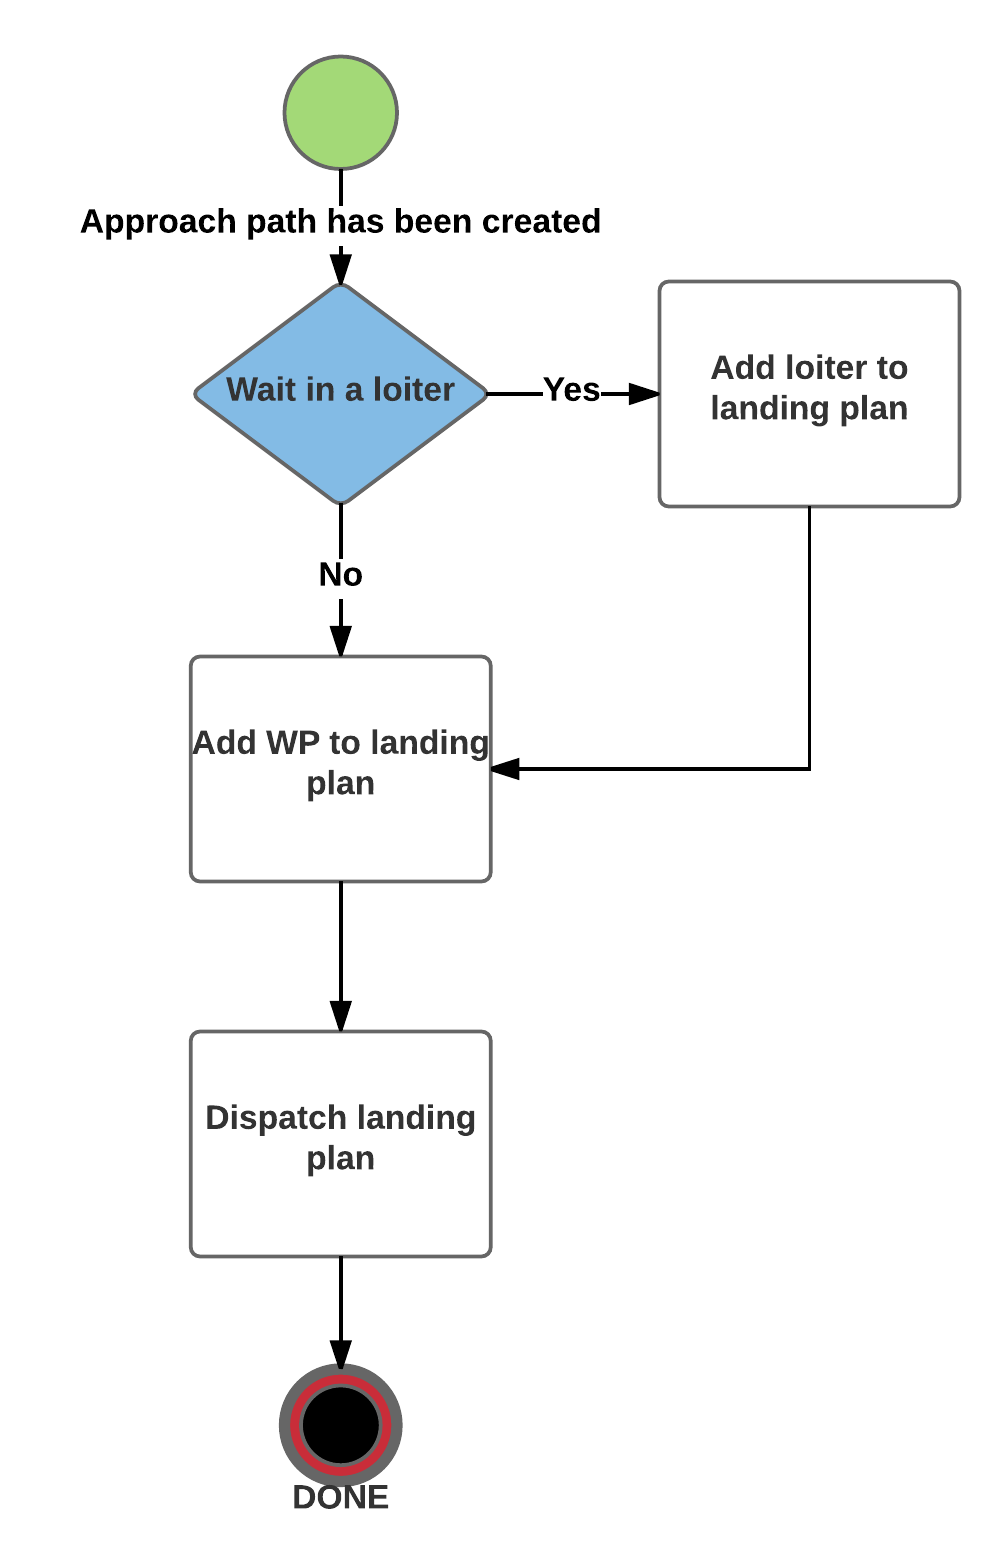
\includegraphics[scale=0.8]{figs/LandingPath.png}
\caption{Flow chart of the landing plan generation}
\label{Fig:FlowChartLanding}
\end{figure}
\section{Testing of software - SIL test}\label{ss:SILLandingPlan}
\subsection{Outline of testing}\label{ss:SILOutline}
The landing plan was verified and test through the use of a \gls{sil} simulation, where the landing plan generation code runs as if it's connected to the actual hardware. The basis for a \gls{sil} test is to perform simulated experimental tests, where the physical part of the system is replaced by a simulator module.  The X8 fixed-wing \gls{uav} is in this case been replaced by the JSBSim simulator module developed by \citep{Gryte}, while the software modules tested represent the actual modules, e.g. the tested modules will not know that the physical system is replaced by software and not the actual \gls{uav}. The result obtain from a simulation is used as a ideal test case, from which the performance of a flight test can be compeered against. However the current model of the X8 used in the simulation has not been completely verified, such that deviation in results and behaviour is expected. Figure \ref{Fig:LandingPathNeptus} shows a screenshot of a landing plan created in Neptus with the green triangle symbolizing the net placement.

The autonomous landing system flies in the Ardupilot mode \gls{fbwa}, where the high level control system is implemented in \gls{dune}. The longitudinal control system during \gls{sil} simulation of the autonomous landing system is designed and tested in the master thesis \citep{Sigurd}, and the lateral control system was design and implemented as part of the paper \citep{fortuna2015cascaded}. A short description of both control system is presented in appendix \ref{AP:ControlGuidanceSystem}. The low level controllers in Ardupilot used in the \gls{sil} simulation are fined tuned for autonomous flight, which allows for ideal test conditions on the performance of the high level controllers. In \gls{dune} the time of arrival factor control when the path control system switches between waypoints, which can be used during turning manoeuvres to force the \gls{uav} to closer follow the path. During the \gls{sil} simulation the time of arrival factor is set to $2 s$.
\begin{figure}[H]
\centering
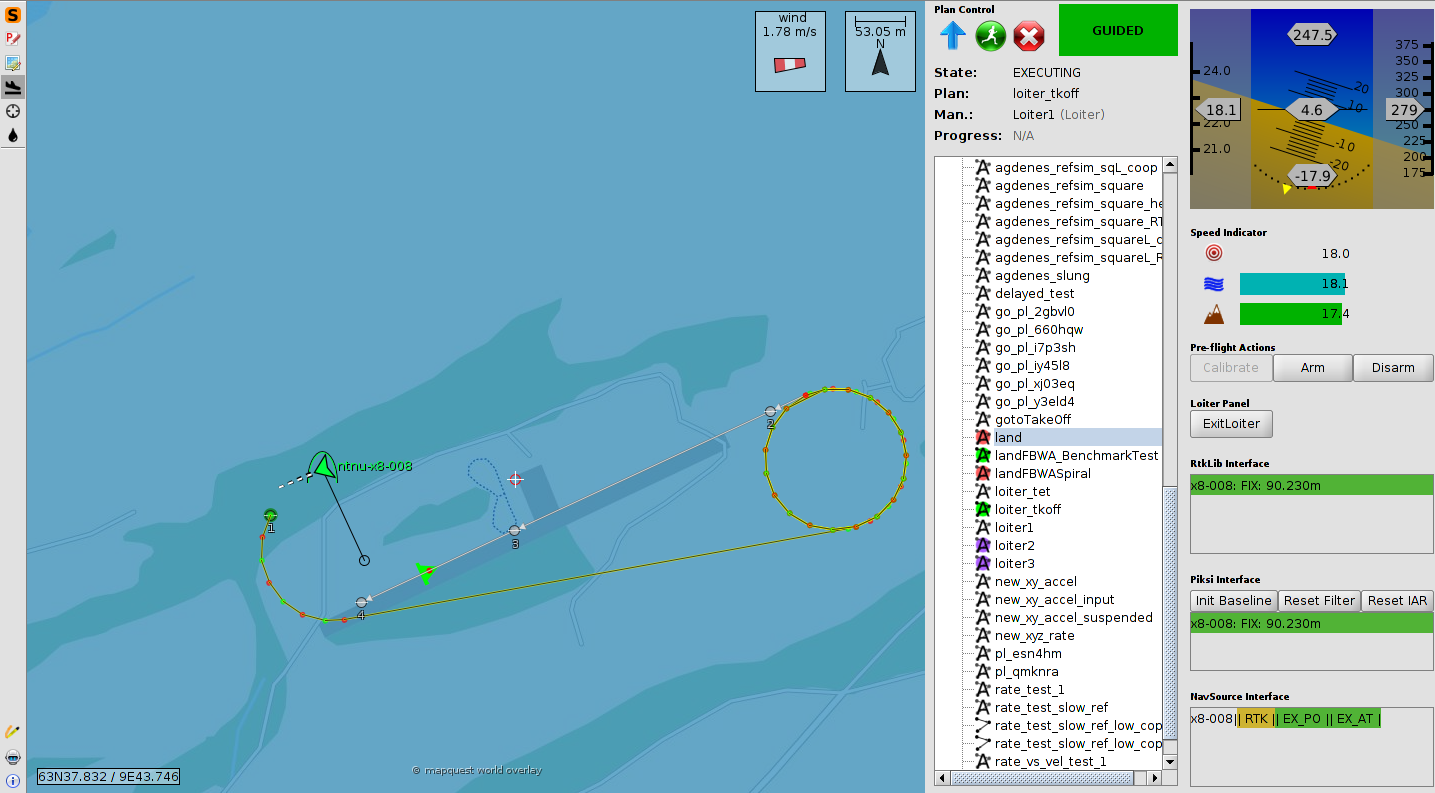
\includegraphics[scale=0.25]{figs/LandingPathNeptus.png}
\caption{Path generated from the landing plan generator, with the net placement as a green triangle}
\label{Fig:LandingPathNeptus}
\end{figure}
\subsection{Landing plan generation}
A landing path was created to simulate a real landing, with the lateral path is shown in figure \ref{Fig:SILNorthEast090145} and the height versus the desired height  shown in figure \ref{Fig:SILHeight6juni090145}. The landing plan is design to fit the operation area in which the fixed wing \gls{uav} can operate during a \gls{los} flight operation.
\begin{figure}[H]
\centering
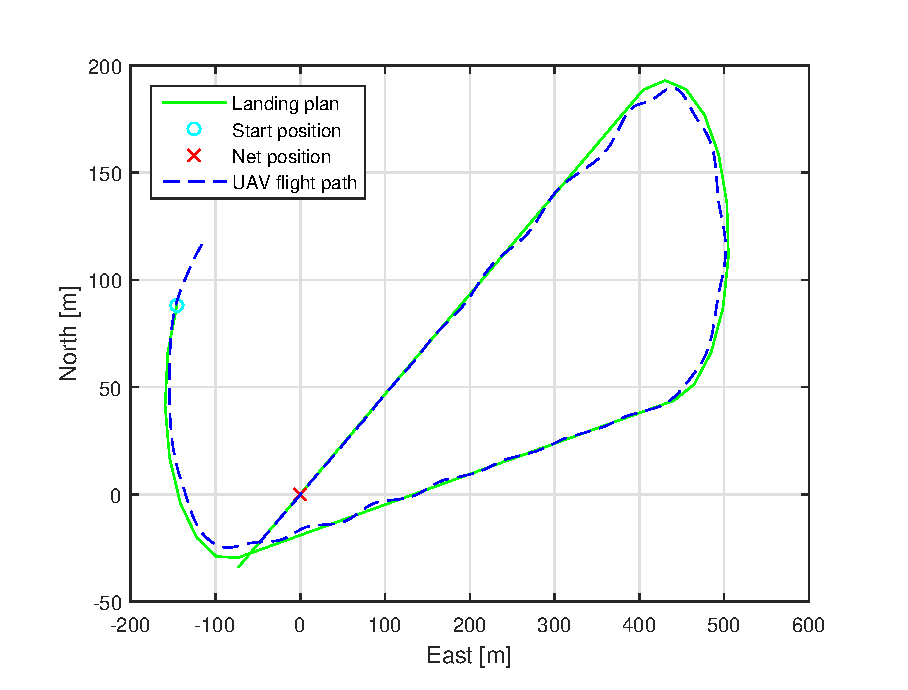
\includegraphics[scale=0.7]{figs/SysPlot/SILNorthEast6juni090145.eps}
\caption{North-East plot of a \gls{sil} simulation of the autonomous landing system.}
\label{Fig:SILNorthEast090145}
\end{figure}
\begin{figure}[H]
\centering
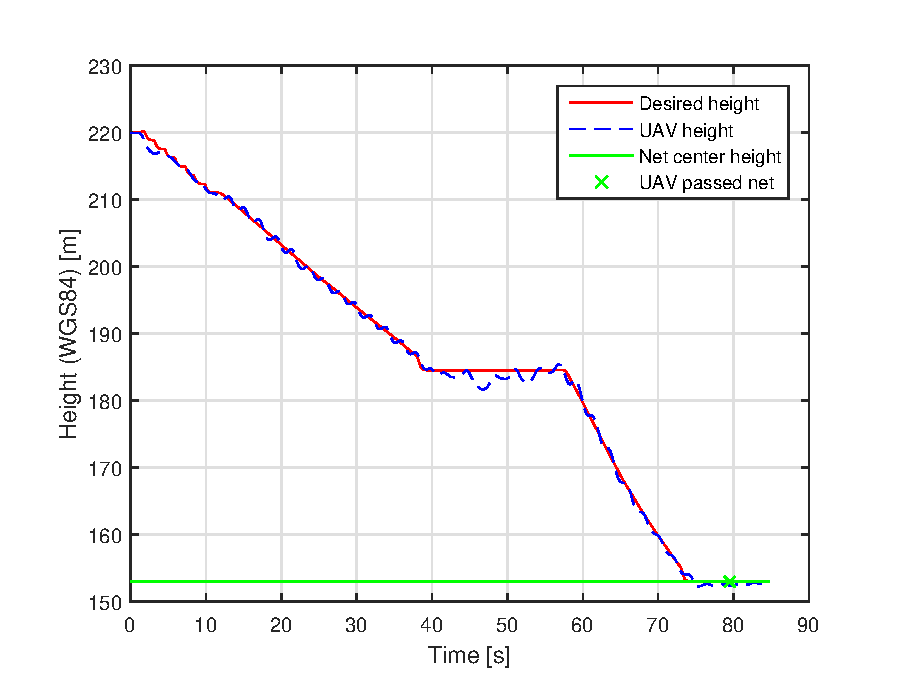
\includegraphics[scale=0.7]{figs/SysPlot/SILHeight6juni090145.eps}
\caption{The desired height and \gls{uav} height when executing the landing plan.}
\label{Fig:SILHeight6juni090145}
\end{figure}
\subsection{Spiral path creation}
During a landing plan the height at the end of the approach path may not match the start height of the landing path. In those cases the spiral path described in section \ref{pp:SpiralPath} is created in order for the approach path to reach the correct height. In figure \ref{Fig:SILNorthEastSpiral092307} the spiral function of the lateral path was tested, with the resulting height profile in figure \ref{Fig:SILHeightSpiral092307}. The simulation was performed with a wind disturbance of $9 m/s$ from the west of the net position, to simulate how the \gls{uav} would perform during the landing plan with wind disturbance. The direction of the wind is set such that the landing path is directed against the wind, which the optimal direction to land in order to reduce the ground speed of the \gls{uav}. 

The lateral control system struggles when flying with the wind, however when flying against the wind it's able to stay on the straight line between the way-points. This is as expected and makes physical sense as the fundamentals of flying is lift created by air velocity over the wing, where the flaps are used to create steering force based on same principle, i.e. air flow over the wing from front to aft with a certain velocity is required to create any steering force/rotational moment. During the turn in the spiral the lateral control system is unable to stay on the circle, thus overshooting the desired path. The longitudinal control system behave similar to the simulation without wind, indicating that as long as the \gls{uav} can fly in the wind the performance from the longitudinal control system would remain the same as with negligible wind conditions.
\newpage
\begin{figure}[H]
\centering
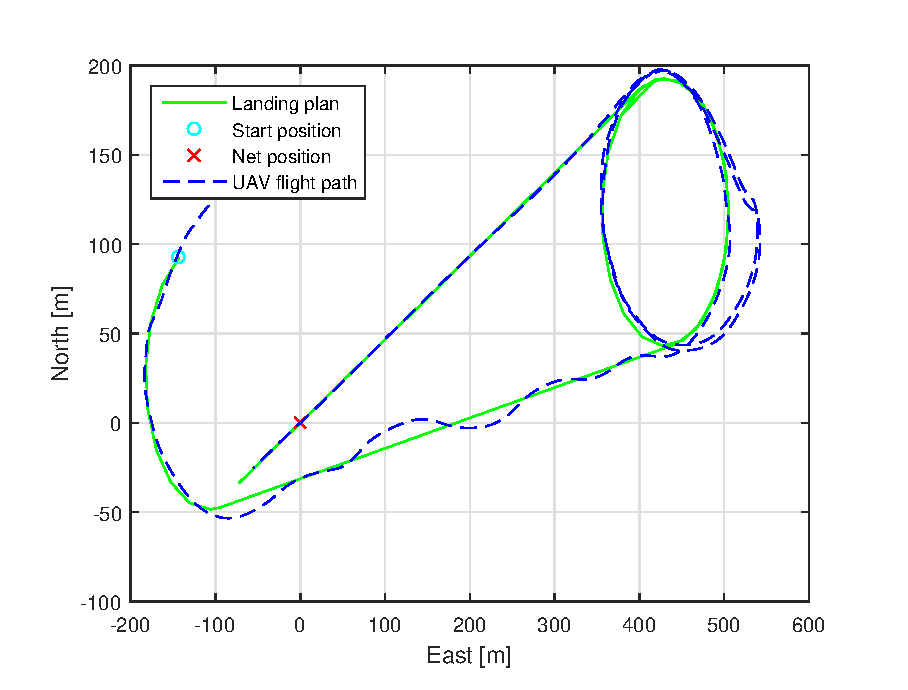
\includegraphics[scale=0.7]{figs/SysPlot/SILNorthEast6juni092307.eps}
\caption{North-East plot where the approach path enters a spiral in order to find a path to the correct height. The simulation was performed with $9 m/s$ wind from west}
\label{Fig:SILNorthEastSpiral092307}
\end{figure}
\begin{figure}[H]
\centering
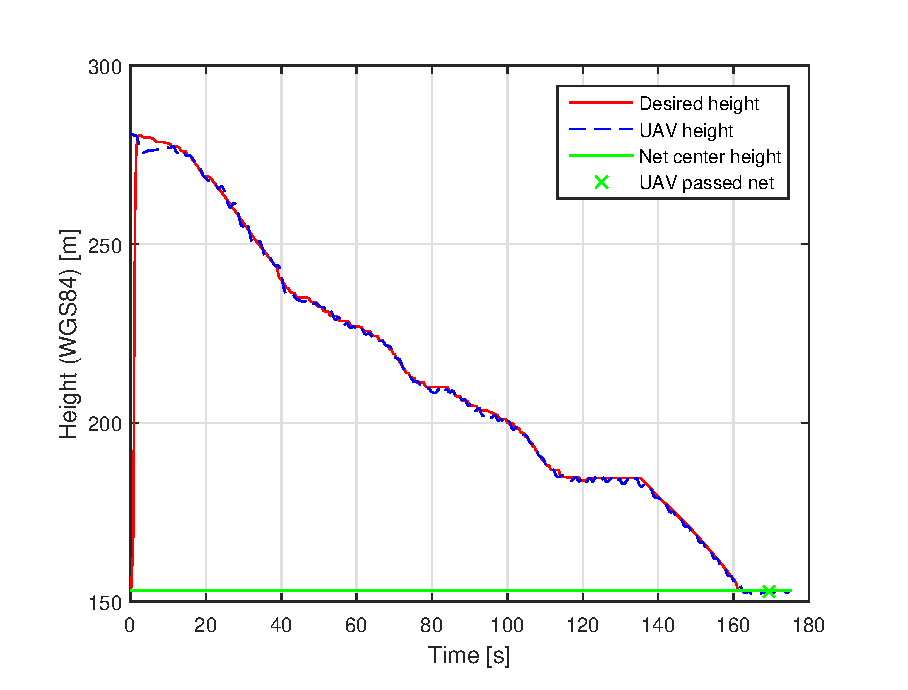
\includegraphics[scale=0.7]{figs/SysPlot/SILHeightSpiral6juni092307.eps}
\caption{The desired height and \gls{uav} height when executing the landing plan from a height that trigger a spiral path towards the correct height with maximum decent angle $\gamma_{d_{Max}}$. The simulation was performed with $9 m/s$ wind from west}
\label{Fig:SILHeightSpiral092307}
\end{figure}
\subsection{Result of simulations}\label{SIL:Results}
The system performance in a simulation environment is presented, where the success criteria is if the \gls{uav} was within the net acceptance criteria at the time the along track error equalled the distance to the aiming point behind the net position. The acceptance criteria used to indicate if the \gls{uav} would have hit the net is given in table \ref{tb:NetCriteria}, which is related to a net with the dimensions 3 meter height and 5 meter width.
\begin{table}[H]
\centering
\begin{tabular}{| l | l |}
\hline
\textbf{Height acceptance}	& \textbf{Cross track error acceptance}	\\ \hline
$\pm1.5$					& $\pm2.5$								\\ \hline
\end{tabular}
\caption{Net hit acceptance criteria}
\label{tb:NetCriteria}
\end{table}
The result from six simulations is given in figure \ref{Fig:SILNetPasing}, with the overall performance of the path following capability of the control system given in table \ref{Tb:SILAverageCrossHeight}. All the simulations of the autonomous landing system gave a result where the \gls{uav} was able to pass the net with a accuracy that is within the acceptance criteria, showing that the system is able to perform autonomous landing. The height difference between the net placement and the start of the landing path was $31.5 m$, where the glide slope angle was set to $6\deg$. A higher glide slope angle would result in the \gls{uav} to build up speed, thus with the current longitudinal control system the angle of the glide slope should not exceed $8\deg$.
\newpage
\begin{figure}[H]
\centering
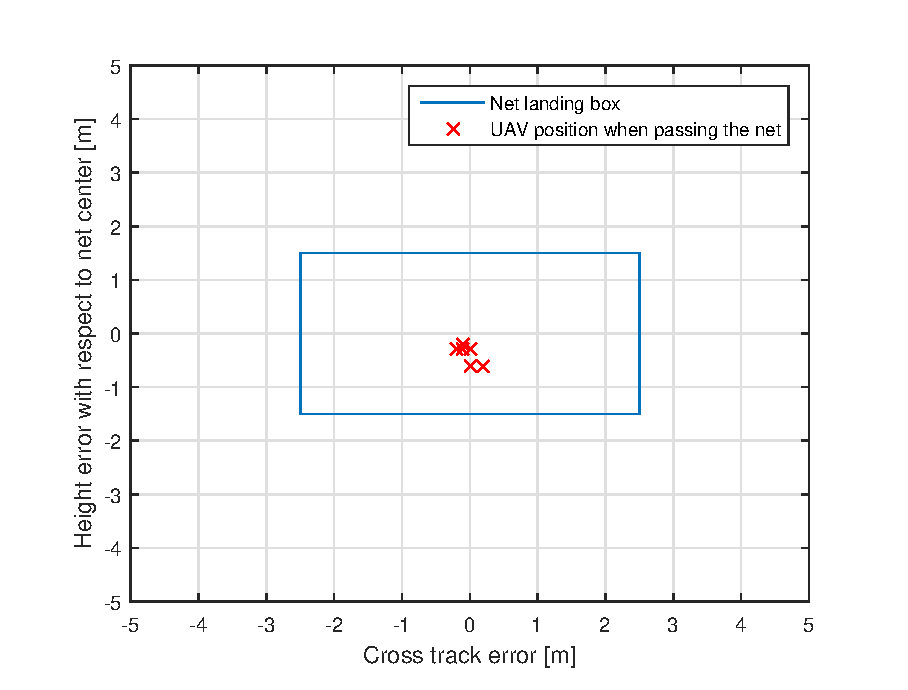
\includegraphics[scale=0.7]{figs/SysPlot/SILNetPasing.eps}
\caption{\gls{uav} position at time of net passing during SIL simulation.}
\label{Fig:SILNetPasing}
\end{figure}
\begin{table}[H]
\centering
\begin{tabular}{| l | l | l |}
\hline
\textbf{Nr.} 	& \textbf{Average height error [m]} 	& \textbf{Average cross track error [m]}  \\ \hline
$1$				& $-0.3$							& $-3.1$								\\ \hline
$2$				& $0.7$							& $-4.0$								\\ \hline
$3$				& $0.2$							& $-3.3$								\\ \hline
$4$				& $0.5$							& $-1.2$								\\ \hline
$5$				& $0.4$							& $-2.5$								\\ \hline
$6$				& $0.2$							& $0.3$								\\ \hline
\end{tabular}
\caption{Average cross track error and height error relative to the path.}
\label{Tb:SILAverageCrossHeight}
\end{table}
\section{Summary}
This chapter has presented the system implementation for the path and navigation system described in chapter \ref{CH:PathNavigation}, as well as presented a mobile sensor unit. The landing plan generator has been tested and verified in a \gls{sil} simulation, together with the control system which will be used in experimental flight tests. The results from the \gls{sil} simulation shows that the system is capable of performing a autonomous landing, however it's expected a deviation in behaviour due to the use of a X8 model that has not been completely verified. In addition the low level controller in the simulator are fined tuned for autonomous flights, which is not the case of the physical X8. The landing path generator is design to be as flexibly as possible when it comes to creating a operational valid landing plan. By having the option of selecting the rotation direction of both the turning circles, a landing plan can be created to suit the surrounding environment to minimize the risk of a crash or the \gls{uav} leave the line of sight. The loiter manoeuvre that included in the landing plan allows a coordination stage, in which the landing zone can be prepared when the \gls{uav} enters the loiter. 

The \gls{uav} navigation system has been design to enable the use of two positioning system, where one is more accurate then the other. The \gls{rtk-gnss} has been made more robust by the creation of a short \gls{rtk-gnss} loss compensator, which apply sensor fusion with navigation data from a secondary \gls{gnss} system in the case of \gls{rtk-gnss} drop out. The navigation source monitor has been design to allow the operator to get a feedback on which navigation source the navigation system is currently using, and which other navigation systems are available.

The mobile sensor unit has been design to function as position reference in Neptus for net placement. The unit comes with it's own \gls{dune} system with \gls{rtk-gnss}, which can be expanded with a closer interaction with the autonomous landing system. However as of today, the net position must either be placed or written in manually in Neptus. An other solution would be that the mobile sensor units position becomes the net position. This would allow for a more advance autonomous landing where target tracking is used by the fixed wing \gls{uav} to land at a offset position above the mobile sensor unit, which is essential in autonomous landing system where the net is dynamical. A similar system has been developed in the master thesis \citep{Jostein}, however here the net is controlled by multirotor \glspl{uav}.
